% Source of MCB2600347_paper_zh_extended.pdf. Build in this folder with two runs of
%   xelatex -jobname=MCB2600347_paper_zh_extended main.tex
% (fonts: TeX Gyre Termes/Heros, STIX Two Math, Noto Serif CJK SC) and copy MCB2600347_paper_zh_extended.pdf to ../
\documentclass[a4paper,11pt]{article}
\usepackage{fontspec}
\setmainfont{TeX Gyre Termes}
\setsansfont{TeX Gyre Heros}
\newfontfamily\cjkfont{Noto Serif CJK SC}
\usepackage{amsmath}
\usepackage{unicode-math}
\setmathfont{STIXTwoMath-Regular.otf}
\usepackage[a4paper,top=2.5cm,bottom=2.4cm,left=2.6cm,right=2.6cm]{geometry}
\usepackage{graphicx,booktabs,array,threeparttable,pdfpages,fancyhdr,xurl}
\usepackage[font=small,labelsep=period,skip=4pt]{caption}
\usepackage[hidelinks,bookmarksnumbered=true,bookmarksopen=true]{hyperref}
\usepackage{titlesec}
\renewcommand{\floatpagefraction}{0.8}\renewcommand{\topfraction}{0.88}\renewcommand{\bottomfraction}{0.7}\renewcommand{\textfraction}{0.1}
\usepackage{etoolbox}\AtBeginEnvironment{thebibliography}{\small\linespread{1.05}\selectfont\setlength{\itemsep}{1pt}\setlength{\parskip}{0pt}}
\setlength{\emergencystretch}{3em}
\linespread{1.15}
\setlength{\parskip}{0.25em}
\titleformat{\section}{\large\bfseries}{E\arabic{section}}{0.8em}{}
\titleformat{\subsection}{\normalsize\bfseries}{E\arabic{section}.\arabic{subsection}}{0.6em}{}
\renewcommand{\thesection}{E\arabic{section}}
\renewcommand{\thefigure}{E\arabic{figure}}
\renewcommand{\thetable}{E\arabic{table}}
\renewcommand{\theequation}{E\arabic{equation}}
\setlength{\headheight}{15pt}\pagestyle{fancy}\fancyhf{}\renewcommand{\headrulewidth}{0.4pt}
\newcommand{\hd}[1]{\begin{tabular}[b]{@{}c@{}}#1\end{tabular}}
\newcommand{\exthead}[1]{\fancyhead[L]{\small #1}\fancyhead[R]{\small Part II\quad Post-competition extensions}\fancyfoot[C]{\small E-\thepage}}

\graphicspath{{../../figures/extension/}}
\hypersetup{pdftitle={Chemistry-driven beer sensory prediction and style design -- extended edition}}
\begin{document}
\thispagestyle{empty}
\begin{center}
{\Large\bfseries Chemistry-Driven Beer Sensory Prediction and Style Design}\\[0.7em]
{\large Extended edition --- note}
\end{center}
\vspace{0.8em}

This file has two parts. Part I is the paper submitted to Problem A of the Big Data track of the 2026 MathorCup Mathematical Application Challenge (73 pages, in Chinese), reproduced exactly as submitted. Part II, starting on page E-1, contains post-competition extensions written in November 2026.

The contest data come from the public study of Schreurs et al.\ in \emph{Nature Communications}. The paper used a different evaluation protocol from that study, so the two sets of $R^2$ values are not directly comparable. E1 reproduces the paper's design, a low-rank branch and an independent-output branch combined by grouped convex fusion, under the study's own protocol: the fusion beats the re-run gradient-boosting benchmark in 9 of 10 splits, and regularised Extra Trees is the strongest single learner. E2 replaces the fusion branches with strong learners and adds a beer-style prior branch, which reaches a macro $R^2$ of 0.238 against 0.21 reported by the study. It also tests the paper's key-compound conclusion against the independent RateBeer consumer ratings in the study's supplementary material: within beer styles, 4-vinylguaiacol is significantly associated with the consumers' clove descriptors.

Every number in Part II can be reproduced with the scripts in the \texttt{extension/} folder of the code repository; result files are in \texttt{results/extension/}.

\clearpage
\pdfbookmark[0]{Part I\quad Competition paper (as submitted)}{part1}
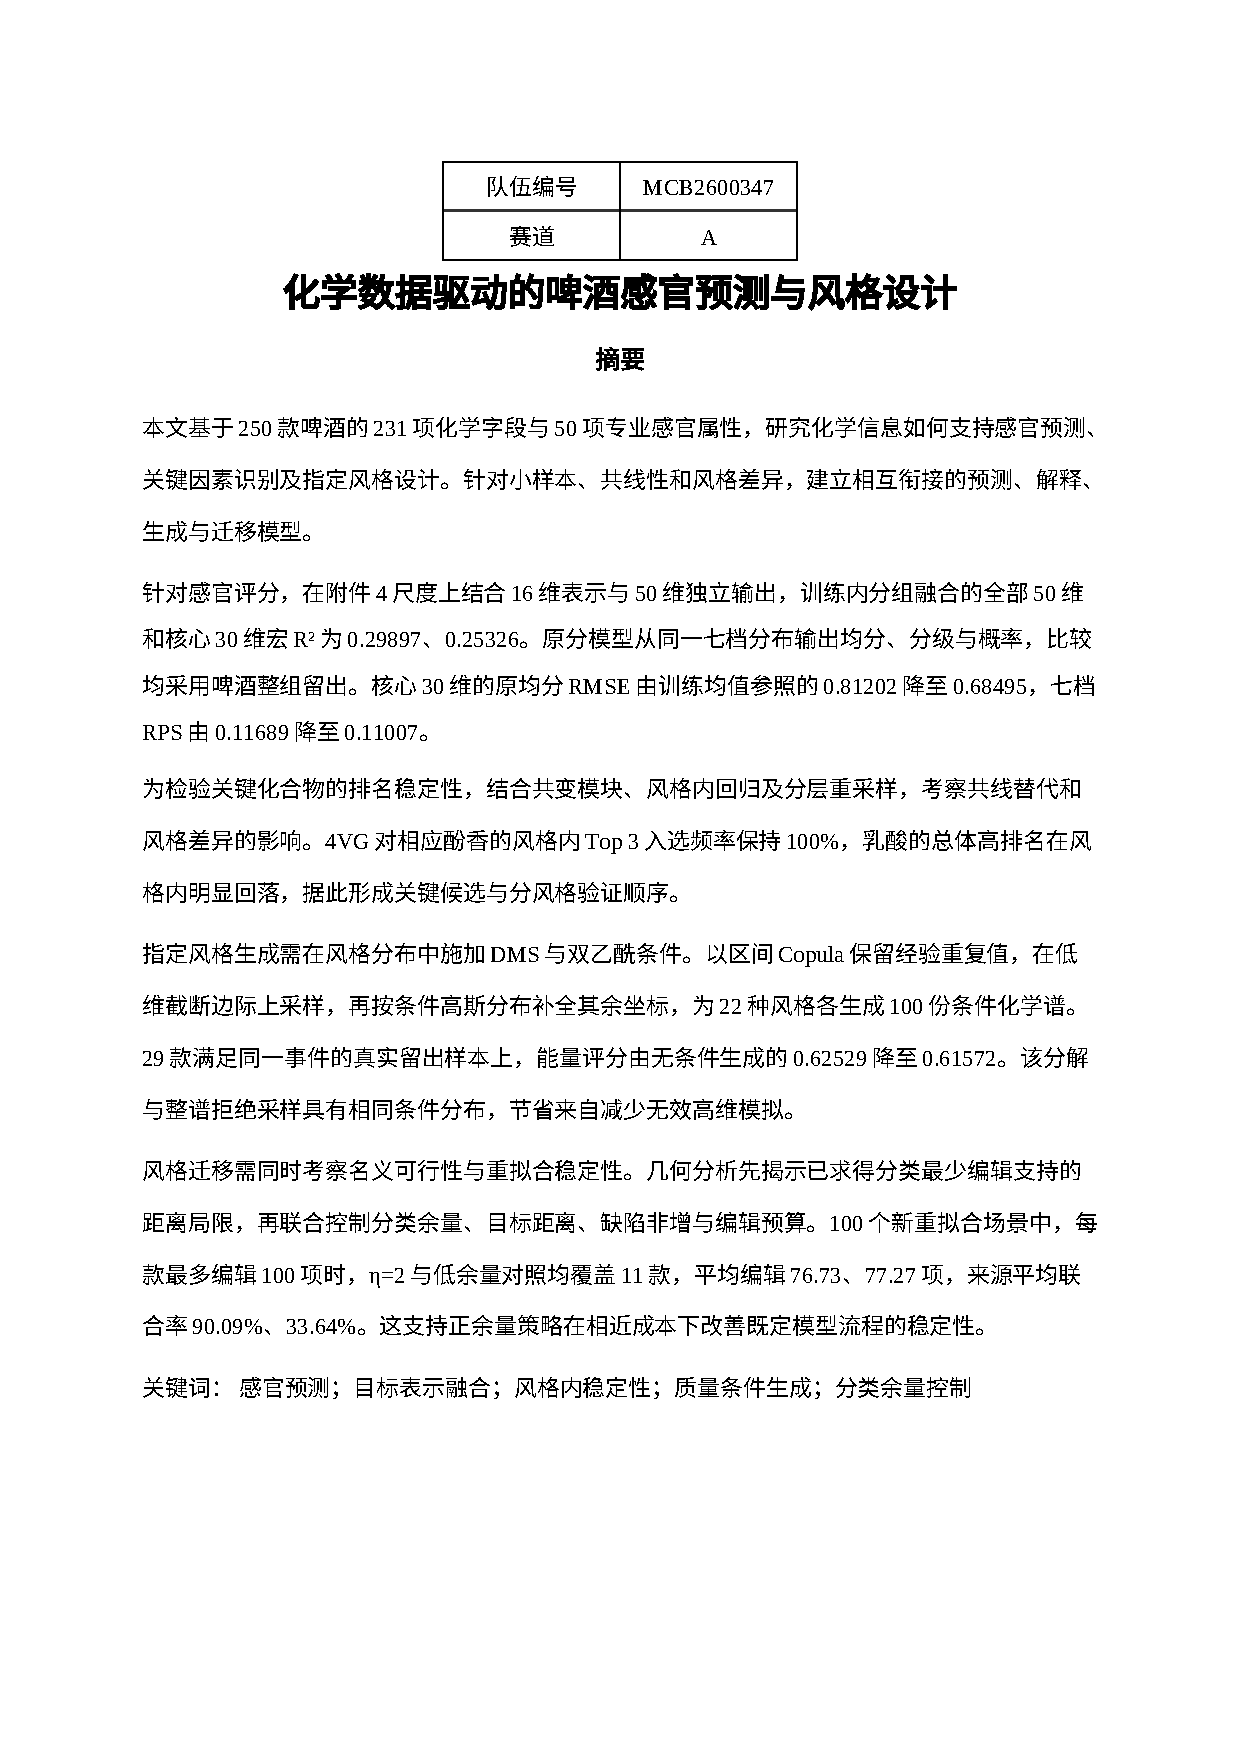
\includepdf[pages=-]{../MCB2600347_paper_zh.pdf}
\pdfbookmark[0]{Part II\quad Post-competition extensions}{part2}
\setcounter{page}{1}
\exthead{Chemistry-driven beer sensory prediction and style design}
\begin{center}{\Large\bfseries Part II\quad Post-competition extensions}\end{center}

From 231 chemical fields and 50 sensory attributes of 250 beers, the paper builds four linked models: prediction, key-compound stability, style-conditioned generation, and sparse style transfer with a classification-margin constraint. The contest data come from the public study of Schreurs et al.\cite{schreurs2024}, whose best model (multi-output gradient-boosting regression, GBR) reports an $R^2$ of 0.21 for the trained-panel attributes on a 70/30 split stratified by beer style. The paper uses a grouped hold-out protocol and the TabICL foundation model, so its numbers cannot be placed directly beside 0.21. Both extensions below use the study's own protocol and the supplementary workbook the study published on Zenodo\cite{zenodo2024}.

\section{The fusion design under the reference study's protocol}

\subsection{Design}
E1 does not use the foundation model and reproduces only the paper's fusion design. Both branches use kernel ridge regression with an RBF kernel; one predicts the 50 outputs independently, the other a 16-dimensional low-rank target. The convex weights of each attribute group are fitted on out-of-fold predictions from a 3-fold split inside the training part. The evaluation uses the study's split (\texttt{random\_state=0}) and 10 further splits stratified by style, and the metric is the macro average of $R^2$ over the 50 attributes.

\subsection{Results}
\begin{table}[htbp]\centering\small
\caption{Macro $R^2$ (50 attributes) under the reference study's protocol.}\label{tab:mc-e1}
\begin{tabular}{lcc}\toprule
Model & Reference split & Mean of 10 splits (s.d.)\\\midrule
GBR, as reported by the study (tuned) & 0.21 & ---\\
GBR, re-run with fixed hyper-parameters & 0.167 & 0.169 (0.030)\\
Kernel ridge, 50 independent outputs & 0.170 & 0.191 (0.022)\\
Kernel ridge, 16-d low-rank target & 0.171 & 0.192 (0.020)\\
\textbf{Grouped convex fusion (paper's design)} & 0.172 & \textbf{0.199 (0.022)}\\
Extra Trees & \textbf{0.222} & \textbf{0.231 (0.019)}\\\bottomrule
\end{tabular}
\end{table}

\begin{figure}[htbp]\centering
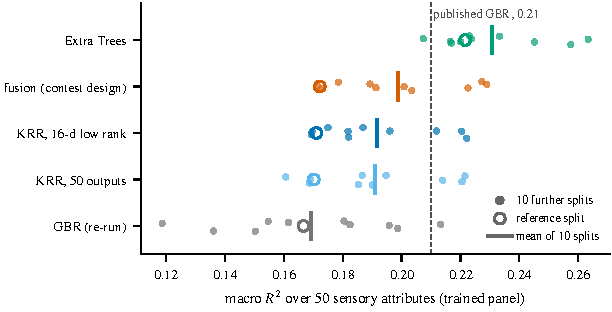
\includegraphics[width=0.66\textwidth]{figE1_published_protocol.pdf}
\caption{Macro $R^2$ of each model under the reference study's protocol (10 stratified splits and the reference split).}\label{fig:mc-e1}
\end{figure}

The fusion step transfers to the new protocol (Table~\ref{tab:mc-e1}, Figure~\ref{fig:mc-e1}). Its mean exceeds that of the better of the two branches by 0.004, the same order as the gains of 0.008--0.019 reported in the paper, and it beats the re-run GBR in 9 of 10 splits (by 0.029 on average). Well-regularised Extra Trees\cite{geurts2006} is the strongest learner under this protocol and exceeds the GBR reported by the study on the reference split (0.222 against 0.21), so replacing kernel ridge with it in the fusion branches is the natural next step. Linear ridge regression is highly unstable under macro $R^2$: individual attributes whose test values are almost constant produce negative $R^2$ values of large magnitude, consistent with the large negative values of the linear models in Supplementary Table S3 of the study. For a 50-dimensional sensory prediction, reporting the macro $R^2$ alone is therefore a fragile summary.

\section{Strong branches, beer style and an external test of the key compound}

\subsection{Design}
Following E1, E2 uses stronger branches under the same protocol, four in total: Extra Trees on the 50 outputs, Extra Trees on the 16-dimensional low-rank target, kernel ridge on the same low-rank target, and a style prior, namely the mean of each attribute over training beers of the same style. The simplex weights of each attribute group are fitted only on out-of-fold predictions inside the training part. All branches are fitted to standardised targets so that the multi-output trees treat the 50 attributes equally; on targets in their original scale (E1), the same Extra Trees configuration scores 0.222 and 0.231.

\subsection{Results}
\begin{table}[htbp]\centering\small
\caption{Fusion of strong branches and the style prior (macro $R^2$, 50 attributes).}\label{tab:mc-e2}
\begin{tabular}{lcc}\toprule
Model & Reference split & Mean of 10 splits (s.d.)\\\midrule
Style prior alone & 0.100 & 0.116 (0.046)\\
Kernel ridge, 16-d low rank & 0.171 & 0.192 (0.020)\\
Extra Trees, 16-d low rank & 0.217 & 0.226 (0.020)\\
Extra Trees, 50 outputs & 0.220 & 0.232 (0.019)\\
Fusion of the three chemistry branches & 0.219 & 0.232 (0.019)\\
\textbf{Fusion including the style prior} & \textbf{0.224} & \textbf{0.238 (0.017)}\\
\emph{GBR, as reported by the study (tuned)} & \emph{0.21} & ---\\\bottomrule
\end{tabular}
\end{table}

The fusion including the style prior sets a new best result under the study's protocol (Table~\ref{tab:mc-e2}). It exceeds Extra Trees by 0.0065 on average (standard error 0.0020) and wins in 9 of 10 splits, and it beats the re-run GBR in all 10 splits (by 0.069 on average). With strong branches the gain comes from beer style rather than from mixing learners: fusing only the chemistry branches ties with Extra Trees, and adding the style prior raises the score by a further 0.006 (in 9 of 10 splits). The style prior alone reaches half of the best macro $R^2$ and receives 22\,\% of the fusion weight on average (27--28\,\% in the aroma and flavour groups, 16--17\,\% in the others), but it is never sufficient: the fusion beats the style prior on all 50 attributes.

\begin{figure}[htbp]\centering
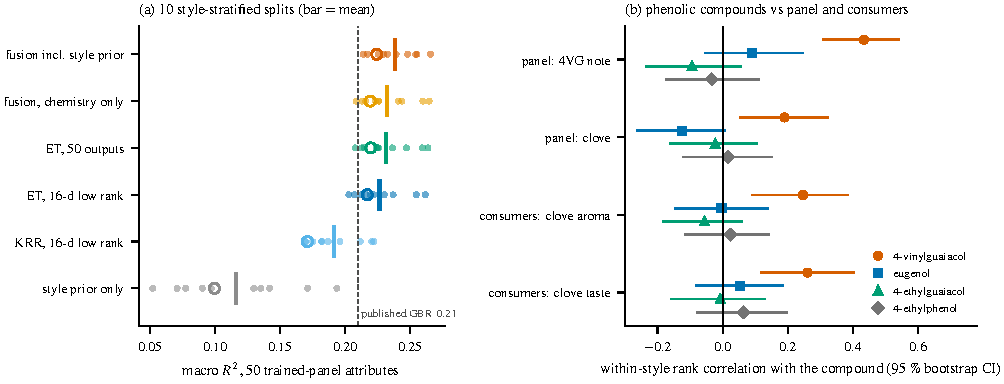
\includegraphics[width=\textwidth]{figE2_strong_fusion_key_compound.pdf}
\caption{(a) Macro $R^2$ on 10 splits stratified by style (points: individual splits; open circles: the reference split; vertical lines: means). (b) Within-style rank correlation of four phenolic compounds with the trained panel's 4VG and clove attributes and with the consumers' clove descriptors (95\,\% intervals from 2\,000 bootstrap resamples).}\label{fig:mc-e2}
\end{figure}

The paper's key-compound conclusion also holds outside the training population. The paper found that 4-vinylguaiacol (4VG) entered the within-style top three for the corresponding phenolic note in 100\,\% of cases. Within beer styles its concentration has a rank correlation of $\rho=0.43$ with that trained-panel attribute (95\,\% interval $[0.31, 0.54]$). More importantly, it is also associated with the ratings of an independent population, the clove descriptors of RateBeer consumers in Supplementary File S7 of the study (aroma 0.25, $[0.09, 0.39]$; taste 0.26, $[0.12, 0.40]$). The other clove-like or smoky phenols measured (eugenol, 4-ethylguaiacol and 4-ethylphenol) show no within-style association with any of the four targets: all 12 intervals contain zero, and the closest to excluding it is eugenol against the panel's clove attribute, $-0.12$ ($[-0.26, 0.01]$).

\subsection{Conclusions and limits}
Under the reference study's protocol the paper's fusion design itself is effective, while what sets the ceiling is the strength of the branch learners and the use of beer style; style information is useful but not sufficient. The paper's key-compound conclusion is supported by independent consumer data. All comparisons rest on the same data for 250 beers: the consumer ratings come from an independent population but refer to the same beers as the panel data, and correlation is not causation, so the effect of 4-vinylguaiacol on clove perception needs to be confirmed by spiking experiments.

\begin{thebibliography}{9}
\bibitem{schreurs2024} M. Schreurs, S. Piampongsant, M. Roncoroni, et al. Predicting and improving complex beer flavor through machine learning. \emph{Nature Communications}, 15: 2368, 2024. doi:10.1038/s41467-024-46346-0.
\bibitem{zenodo2024} M. Schreurs, S. Piampongsant, M. Roncoroni, et al. Data from: Predicting and improving complex beer flavor through machine learning. Zenodo, 2024. doi:10.5281/zenodo.10653704.
\bibitem{geurts2006} P. Geurts, D. Ernst, L. Wehenkel. Extremely randomized trees. \emph{Machine Learning}, 63(1): 3--42, 2006. doi:10.1007/s10994-006-6226-1.
\end{thebibliography}
\end{document}
